
%{{第十四回}}{第十四回}}

\chapter{林如海捐馆扬州城\\贾宝玉路谒北静王}\label{part0018_split_000.htmlux5cux23calibre_pb_0}

{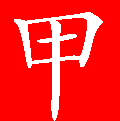
\includegraphics[width=3mm]{../Images/00002}凤姐用彩明,因自识字不多,且彩明系未冠之童。}

{写凤姐之珍贵,写凤姐之英气,写凤姐之声势,写凤姐之心机,写凤姐之骄大。}

{昭儿回,并非林文、琏文,是黛玉正文。}

{牛,丑也。清属水,子也。柳拆卯字。彪拆虎字,寅字寓焉。陈即辰。翼火为蛇,巳字寓焉。马,午也。魁拆鬼,鬼,金羊,未字寓焉。侯、猴同音,申也。晓鸣,鸡也,酉字寓焉。石即豕,亥字寓焉。其祖曰守业,即守夜也,犬字寓焉。此所谓十二支寓焉。}

{路谒北静王,是宝玉正文。}

{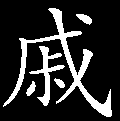
\includegraphics[width=3mm]{../Images/00005}家书一纸千金重,勾引难防嘱下人。任你无双肝胆烈,多情念起自眉颦。}

诗云:\ldots{}\ldots{}

话说宁国府中都总管来升闻得里面委请了凤姐,因传齐同事人等说道:``如今请了西府里琏二奶奶管理内事。倘或他来支取东西或是说话,我们须要比往日小心些。每日大家早来晚散,宁可辛苦这一个月,过后再歇着,不要把老脸面丢了。{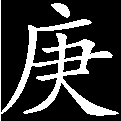
\includegraphics[width=3mm]{../Images/00004}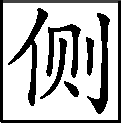
\includegraphics[width=3mm]{../Images/00011}\footnotesize \kaishu 此是都总管的话头。}那是个有名的烈货,脸酸心硬,一时恼了不认人的。''众人都道:``有理。''又有一个笑道:``论理,我们里面也须得他来整治整治,{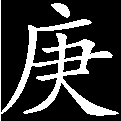
\includegraphics[width=3mm]{../Images/00004}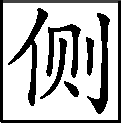
\includegraphics[width=3mm]{../Images/00011}\footnotesize \kaishu 伏线在二十板之误差妇人。}都特不像了。''正说着,只见来旺媳妇拿了对牌,来领取呈文、京榜纸札,票上批着数目。众人连忙让坐倒茶,一面命人按数取纸来抱着,同来旺媳妇一路行来,至仪门口,方交与来旺媳妇自己抱进去了。

凤姐即命彩明定造簿册。{{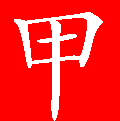
\includegraphics[width=3mm]{../Images/00002}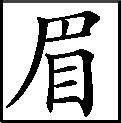
\includegraphics[width=3mm]{../Images/00010}\footnotesize \kaishu 宁府如此大家,阿凤如此身份,岂有使贴身丫头与家里男人答话交事之理呢?此作者忽略之处。 }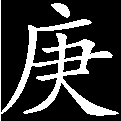
\includegraphics[width=3mm]{../Images/00004}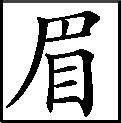
\includegraphics[width=3mm]{../Images/00010}\footnotesize \kaishu 彩明系未冠小童,阿凤便于出入使令者。老兄并未前后看明是男是女,乱加批驳。可笑。◇{且明写阿凤不识字之故。壬午春。}}即时传来升媳妇,兼要家口花名册来查看,又限于明日一早传齐家人媳妇进来听差等语。大概点了一点数目单册,{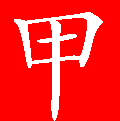
\includegraphics[width=3mm]{../Images/00002}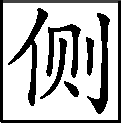
\includegraphics[width=3mm]{../Images/00011}\footnotesize \kaishu 已有成见。}问了来升媳妇几句话,便坐了车回家。一宿无话。

至次日,卯正二刻便过来了。那宁国府中婆娘媳妇闻得到齐,只见凤姐正与来升媳妇分派,众人不敢擅入,只在窗外听觑。{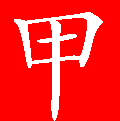
\includegraphics[width=3mm]{../Images/00002}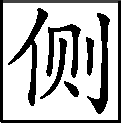
\includegraphics[width=3mm]{../Images/00011}\footnotesize \kaishu 传神之笔。}只听凤姐与来升媳妇道:``既托了我,我就说不得要讨你们嫌了。{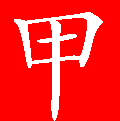
\includegraphics[width=3mm]{../Images/00002}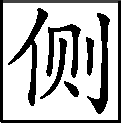
\includegraphics[width=3mm]{../Images/00011}\footnotesize \kaishu 先站地步。}我可比不得你们奶奶好性儿,由着你们去,再不要说你们这府里`原是这样的',{{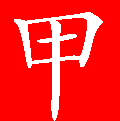
\includegraphics[width=3mm]{../Images/00002}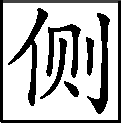
\includegraphics[width=3mm]{../Images/00011}\footnotesize \kaishu 此话听熟了。一叹! }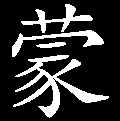
\includegraphics[width=3mm]{../Images/00006}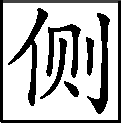
\includegraphics[width=3mm]{../Images/00011}\footnotesize \kaishu ``不要说`原是这样'的话'',破尽痼弊根底。}这如今可要依着我,{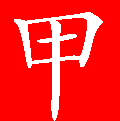
\includegraphics[width=3mm]{../Images/00002}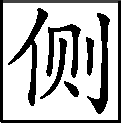
\includegraphics[width=3mm]{../Images/00011}\footnotesize \kaishu 婉转得妙!}行错我半点儿,管不得谁是有脸的,谁是没脸的,一例现清白处治!''说着,便吩咐彩明念花名册,按名一个一个的唤进来看视。{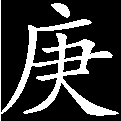
\includegraphics[width=3mm]{../Images/00004}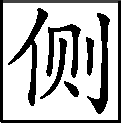
\includegraphics[width=3mm]{../Images/00011}\footnotesize \kaishu 量才而用之意。}

一时看完了,便又吩咐道:``这二十个分作两班,一班十个,每日在里头单管人来客往倒茶,别的事不用他们管。这二十个也分两班,每日单管本家亲戚茶饭,别的事也不用他们管。这四十个人也分作两班,单在灵前上香添油、挂幔守灵、供饭供茶、随起举哀,别的事也不与他们相干。这四个人单在内茶房收管杯碟茶器,若少一件,便叫他四个人描赔。这四个人单管酒饭器皿,少一件,也是他四个人描赔。这八个人单管监收祭礼。这八个人单管各处灯油、蜡烛、纸札,我总支了来,交与你八个,然后按我的定数再往各处去分派。这三十个每日轮流各处上夜,照管门户,监察火烛,打扫地方。这下剩的按着房屋分开,某人守某处,某处所有桌椅、古董起,至于痰盒掸帚,一草一苗,或丢或坏,就和守这处的人算账描赔。来升家的每日揽总查看,或有偷懒的,赌钱吃酒的,打架拌嘴的,立刻来回我。你有徇情,经我查出,三四辈子的老脸就顾不成了。如今都有了定规,以后那一行乱了,只和那一行说话。素日跟我的,随身自有钟表,不论大小事,我是皆有一定的时辰。横竖你们上房里也有时辰钟。卯正二刻我来点卯,巳正吃早饭,凡有领牌、回事的,只在午初刻。戌初烧过黄昏纸,我亲到各处查一遍,回来上夜的交明钥匙。第二日还是卯正二刻过来。说不得咱们大家辛苦这几日,{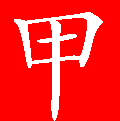
\includegraphics[width=3mm]{../Images/00002}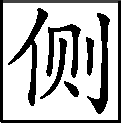
\includegraphics[width=3mm]{../Images/00011}\footnotesize \kaishu 是协理口气,好听之至! 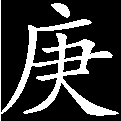
\includegraphics[width=3mm]{../Images/00004}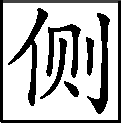
\includegraphics[width=3mm]{../Images/00011}\footnotesize \kaishu 所谓先礼后兵是也。}事完,你们家大爷自然赏你们。''{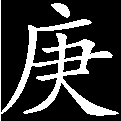
\includegraphics[width=3mm]{../Images/00004}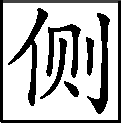
\includegraphics[width=3mm]{../Images/00011}\footnotesize \kaishu 滑贼,好收煞。}

说毕,又吩咐按数发与茶叶、油烛、鸡毛掸子、笤帚等物。一面又搬取家伙------桌围、椅搭、坐褥、毡席、痰盒、脚踏之类,一面交发,一面提笔登记,某人管某处,某人领某物,开得十分清楚。众人领了去,也都有了投奔,不似先时只拣便宜的做,剩下苦差没个招揽。各房中也不能趁乱失迷东西。便是人来客往,也都安静了,不比先前正摆茶又去端饭,正陪举哀又顾接客。如这些无头绪、荒乱、推托、偷闲、窃取等弊,次日一概都蠲了。

凤姐儿见自己威重令行,心中十分得意。因见尤氏犯病,贾珍又过于悲哀,不大进饮食,自己每日从那府里煎了各色细粥、精致小菜,命人送来劝食。{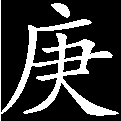
\includegraphics[width=3mm]{../Images/00004}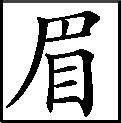
\includegraphics[width=3mm]{../Images/00010}\footnotesize \kaishu 写凤之心机。}贾珍也另外吩咐每日送上等菜到抱厦内,单与凤姐吃。{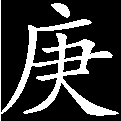
\includegraphics[width=3mm]{../Images/00004}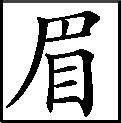
\includegraphics[width=3mm]{../Images/00010}\footnotesize \kaishu 写凤之珍贵。}那凤姐不畏勤劳,{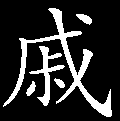
\includegraphics[width=3mm]{../Images/00005}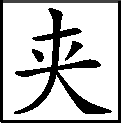
\includegraphics[width=3mm]{../Images/00012}\footnotesize \kaishu 不畏勤劳者,一则任专而易办,一则技痒而莫遏。士为知己者死。不过勤劳,有何可畏?}天天于卯正二刻就过来点卯理事,{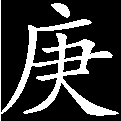
\includegraphics[width=3mm]{../Images/00004}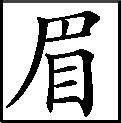
\includegraphics[width=3mm]{../Images/00010}\footnotesize \kaishu 写凤之英勇。}独在抱厦内起坐,不与众妯娌合群,便有堂客来往,也不迎会。{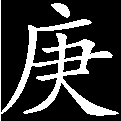
\includegraphics[width=3mm]{../Images/00004}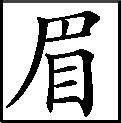
\includegraphics[width=3mm]{../Images/00010}\footnotesize \kaishu 写凤之骄大。}

这日,正五七正五日上,那应{{(佛)}}{[}赴{]}僧正开方破狱,传灯照亡,参阎君,拘都鬼,延请地藏王,开金桥,引幢幡;那道士们正伏章申表,朝三清,叩玉帝;禅僧们行香,放焰口,拜水忏;又有十三众青年尼僧,搭绣衣,靸红鞋,在灵前默诵接引诸咒,十分热闹。{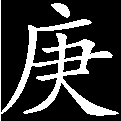
\includegraphics[width=3mm]{../Images/00004}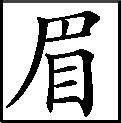
\includegraphics[width=3mm]{../Images/00010}\footnotesize \kaishu 如此写得可叹可笑。}那凤姐必知今日人客不少,在家中歇宿一夜,至寅正,平儿便请起来梳洗。及收拾完备,更衣盥手,吃了两口奶子糖粳粥,漱口已毕,已是卯正二刻了。来旺媳妇率领诸人伺候已久。凤姐出至厅前,上了车,前面打了一对明角灯,大书``荣国府''三个大字,款款来至宁府。大门上门灯朗挂,两边一色戳灯照如白昼,白茫茫穿孝仆从两边侍立。请车至正门上,小厮等退去,众媳妇上来揭起车帘。凤姐下了车,一手扶着丰儿,两个媳妇执着手把灯罩,簇拥着凤姐进来。宁府诸媳妇迎来请安接待。凤姐缓缓走入会芳园中登仙阁灵前,一见了棺材,那眼泪恰似断线珍珠滚将下来。院中许多小厮垂手伺候烧纸。凤姐吩咐得一声:``供茶,烧纸。''只听得一棒锣鸣,诸乐齐奏,{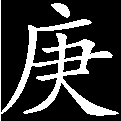
\includegraphics[width=3mm]{../Images/00004}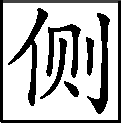
\includegraphics[width=3mm]{../Images/00011}\footnotesize \kaishu 谁家行事?宁不堕泪!}早有人端过一张大圈椅来,放在灵前,凤姐坐了,放声大哭。于是里外男女上下,见凤姐出声,都忙接声嚎哭。

一时贾珍、尤氏遣人来劝,凤姐方才止住。来旺媳妇献茶漱口毕,凤姐方起身,别过族中诸人,自入抱厦内来,按名查点,各项人数都已到齐,只有迎送亲客上的一人未到。{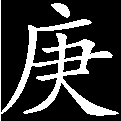
\includegraphics[width=3mm]{../Images/00004}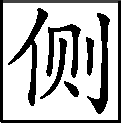
\includegraphics[width=3mm]{../Images/00011}\footnotesize \kaishu 须得如此,方见文章妙用。余前批非谬。}即命传到。那人已张惶愧惧。凤姐冷笑{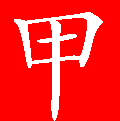
\includegraphics[width=3mm]{../Images/00002}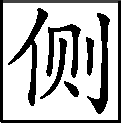
\includegraphics[width=3mm]{../Images/00011}\footnotesize \kaishu 凡凤姐恼时,偏偏用``笑''字,是章法。}道:``我说是谁误了,原来是你!{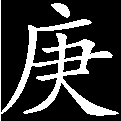
\includegraphics[width=3mm]{../Images/00004}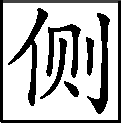
\includegraphics[width=3mm]{../Images/00011}\footnotesize \kaishu 四字有神,是有名姓上等人口气。}你原比他们有体面,所以才不听我的话。''那人道:``小的天天来的早,只有今日醒了觉得早些,因又睡迷了,来迟了一步,求奶奶饶过这次。''正说着,只见荣国府中的王兴媳妇来了,{\includegraphics[width=3mm]{../Images/00002}\includegraphics[width=3mm]{../Images/00011}\footnotesize \kaishu 惯起波澜,惯能忙中写闲,又惯用曲笔,又惯综错,真妙! \includegraphics[width=3mm]{../Images/00004}\includegraphics[width=3mm]{../Images/00011}\footnotesize \kaishu 偏用这等闲文间住。}在前面探头。

凤姐且不发放这人,{{\includegraphics[width=3mm]{../Images/00004}\includegraphics[width=3mm]{../Images/00011}\footnotesize \kaishu 的是凤姐作{(仿)}{[}派{]}。}}却先问:``王兴媳妇作什么?''王兴媳妇巴不得先问他完了事,连忙进来说:``领牌取线,打车轿网络。''{\includegraphics[width=3mm]{../Images/00004}\includegraphics[width=3mm]{../Images/00011}\footnotesize \kaishu 是丧事中用物,闲闲写却。}说着,将个帖儿递上去。凤姐命彩明念道:``大轿两顶,小轿四顶,车四辆,共用大小络子若干根,用珠儿线若干斤。''凤姐听了,数目相合,便命彩明登记,取荣府对牌掷下。王兴家的去了。

凤姐方欲说话时,只见荣府四个执事人进来,都是要支取东西领牌来的。凤姐命彩明要了帖儿念过,听了共四件,凤姐因指两件说道:``这两件开销错了,再算清了来取。''{\includegraphics[width=3mm]{../Images/00004}\includegraphics[width=3mm]{../Images/00011}\footnotesize \kaishu 好看煞,这等文字。}说着掷下帖子来。那二人扫兴而去。

凤姐因见张材家的在旁,{\includegraphics[width=3mm]{../Images/00004}\includegraphics[width=3mm]{../Images/00011}\footnotesize \kaishu 又一顿挫。}因问:``你有什么事?''张材家的忙取帖儿回说道:``就是方才车轿围做成,领取裁缝工银若干两。''凤姐听了,便收了帖子,命彩明登记,待王兴家的交过牌,得了买办的回押,相符,然后方与张材家的去领。一面又命念那一个,是为宝玉外书房完竣,支买纸料糊裱。{\includegraphics[width=3mm]{../Images/00004}\includegraphics[width=3mm]{../Images/00011}\footnotesize \kaishu 却从闲中又引出一件关系文字乎?}凤姐听了,即命收帖儿登记,待张材家的缴清,又发与这人去了。

凤姐便说道:``明儿他也睡迷了,后儿我也睡迷了,{\includegraphics[width=3mm]{../Images/00002}\includegraphics[width=3mm]{../Images/00011}\footnotesize \kaishu 接上文,一点痕迹俱无,且是仍与方才诸人说话神色口角。 \includegraphics[width=3mm]{../Images/00004}\includegraphics[width=3mm]{../Images/00011}\footnotesize \kaishu 接得紧,且无痕迹,是山断云连法也。}将来都没有人了。本来要饶你,只是我头一次宽了,下次人就难管,不如开发的好。''登时放下脸来,喝命:``带出去,打二十大板!''一面又掷下宁府对牌:``出去说与来升,革他一月银米!''众人听了,又见凤姐眉立,{\includegraphics[width=3mm]{../Images/00004}\includegraphics[width=3mm]{../Images/00011}\footnotesize \kaishu 二字如神。}知是恼了,不敢怠慢,拖人的出去拖人,执牌传谕的忙去传谕。那人身不由己,已拖出去挨了二十大板,还要进来叩谢。凤姐道:``明儿再有误的打四十,后日的六十,有不怕打的只管误!''说着,吩咐:``散了罢。''窗外众人听说,方各自执事去了。彼时荣国、宁国两处执事领牌交牌的人来往不绝,那抱愧被打之人含羞去了,这才知道凤姐的利害。{\includegraphics[width=3mm]{../Images/00002}\includegraphics[width=3mm]{../Images/00011}\footnotesize \kaishu 又伏下文,非独为阿凤之威势费此一段笔墨。}众人不敢偷安,自此兢兢业业,{\includegraphics[width=3mm]{../Images/00004}\includegraphics[width=3mm]{../Images/00011}\footnotesize \kaishu 收拾得好。}执事保守,不在话下。

如今且说宝玉{\includegraphics[width=3mm]{../Images/00004}\includegraphics[width=3mm]{../Images/00011}\footnotesize \kaishu 忙中闲笔。}因见今日人众,恐秦钟受了委曲,因默与他商议,要同他往凤姐处来坐。秦钟道:``他的事多,况且不喜人去,咱们去了,他岂不烦腻?''{\includegraphics[width=3mm]{../Images/00002}\includegraphics[width=3mm]{../Images/00011}\footnotesize \kaishu 纯是体贴人情。}宝玉道:``他怎好腻我们,不相干,只管跟我来。''说着,便拉了秦钟,直至抱厦。凤姐才吃饭,见他们来了,便笑道:``好长腿子,快上来罢。''宝玉道:``我们偏了。''{\includegraphics[width=3mm]{../Images/00004}\includegraphics[width=3mm]{../Images/00011}\footnotesize \kaishu 家常戏言,毕肖之至!}凤姐道:``在这边外头吃的,还是那边吃的?''宝玉道:``这边同那些浑人{\includegraphics[width=3mm]{../Images/00002}\includegraphics[width=3mm]{../Images/00011}\footnotesize \kaishu 奇称。试问谁是清人?}吃什么!原是那边,我们两个同老太太吃了来的。''一面归座。

凤姐吃毕饭,就有宁国府中的一个媳妇来领牌,为支取香灯事。凤姐笑道:``我算着你们今日该来支取,总不见来,想是忘了。这会子到底来取,要忘了,自然是你们包出来,都便宜了我。''那媳妇笑道:``何尝不是忘了,{\includegraphics[width=3mm]{../Images/00002}\includegraphics[width=3mm]{../Images/00011}\footnotesize \kaishu 此妇亦善迎合。 \includegraphics[width=3mm]{../Images/00004}\includegraphics[width=3mm]{../Images/00011}\footnotesize \kaishu 下人迎合凑趣,毕真。}方才想起来。再迟一步,也领不成了。''说罢,领牌而去。

一时登记交牌。秦钟因笑道:``你们两府里都是这牌,倘或别人私弄一个,支了银子跑了,怎样?''{\includegraphics[width=3mm]{../Images/00004}\includegraphics[width=3mm]{../Images/00011}\footnotesize \kaishu 小人语。}凤姐笑道:``依你说,都没王法了。''宝玉道:``怎么咱们家没人来领牌子做东西?''{\includegraphics[width=3mm]{../Images/00004}\includegraphics[width=3mm]{../Images/00011}\footnotesize \kaishu 写不理家务公子之语。}凤姐道:``人家来领的时候,你还做梦呢。{\includegraphics[width=3mm]{../Images/00004}\includegraphics[width=3mm]{../Images/00011}\footnotesize \kaishu 言甚是也。}我且问你,你们这夜书多早晚才念呢?''{\includegraphics[width=3mm]{../Images/00004}\includegraphics[width=3mm]{../Images/00011}\footnotesize \kaishu 补前文之未到。}宝玉道:``巴不得这如今就念才好,他们只是不快收拾出书房来,这也没法。''凤姐笑道:``你请我一请,包管就快了。''宝玉道:``你要快也不中用。他们该作到那里的,自然就有了。''凤姐笑道:``便是他们作,也得要东西去,搁不住我不给对牌是难的。''宝玉听说,便猴{\includegraphics[width=3mm]{../Images/00004}\includegraphics[width=3mm]{../Images/00011}\footnotesize \kaishu 诗中知有炼字一法,不期于《石头记》中多得其妙。}向凤姐身上立刻要牌,说:``好姐姐,给出牌子来,叫他们要东西去。''凤姐道:``我乏的身上生疼,还搁的住你揉搓。你放心罢,今儿才领了纸裱糊去了。他们该要的,还等叫去呢,可不傻了?''宝玉不信,凤姐便叫彩明查册子与宝玉看了。

正闹着,人回:``苏州去的人昭儿来了。''{\includegraphics[width=3mm]{../Images/00002}\includegraphics[width=3mm]{../Images/00011}\footnotesize \kaishu 接得好!}凤姐急命唤进来。昭儿打千请安。凤姐儿便问:``回来做什么?''昭儿道:``二爷打发回来的。林姑老爷是九月初三日巳时没的。{\includegraphics[width=3mm]{../Images/00002}\includegraphics[width=3mm]{../Images/00010}\footnotesize \kaishu 颦儿方可长居荣府之文。}二爷带了林姑娘{\includegraphics[width=3mm]{../Images/00004}\includegraphics[width=3mm]{../Images/00011}\footnotesize \kaishu 暗写黛玉。}同送林姑老爷的灵到苏州,大约赶年底就回来了。二爷打发小的来报个信请安,讨老太太示下,还瞧瞧奶奶家里好,叫把大毛衣服带几件去。''凤姐道:``你见过别人了没有?''昭儿道:``都见过了。''说毕,连忙退出。凤姐向宝玉笑道:``你林妹妹可在咱们家住长了。''{\includegraphics[width=3mm]{../Images/00004}\includegraphics[width=3mm]{../Images/00011}\footnotesize \kaishu 此系无意中之有意,妙!}宝玉道:``了不得!想来这几日他不知哭的怎么样呢!''说着蹙眉长叹。

凤姐见昭儿回来,因当着人未及细问贾琏,心中自是记挂。待要回去,争奈事情繁杂,一时去了恐有延迟失误,惹人笑话。少不得耐到晚上回来,复命昭儿进来,细问一路平安信息。连夜打点大毛衣服,和平儿亲自检点包裹,再细细追想所需{\includegraphics[width=3mm]{../Images/00006}\includegraphics[width=3mm]{../Images/00011}\footnotesize \kaishu ``追想所需''四字,写尽能事者之所以{[}为{]}能事者之底蕴。}何物,一并包藏交付。又细细吩咐昭儿``在外好生小心伏侍,不要惹你二爷生气;时时劝他少吃酒,别勾引他认得浑账女人,{\includegraphics[width=3mm]{../Images/00002}\includegraphics[width=3mm]{../Images/00011}\footnotesize \kaishu 切心事耶。}回来打折你的腿''{\includegraphics[width=3mm]{../Images/00002}\includegraphics[width=3mm]{../Images/00011}\footnotesize \kaishu 此一句最要紧。}等语。赶乱完了,天已四更将尽,纵睡下,又走了困,{\includegraphics[width=3mm]{../Images/00004}\includegraphics[width=3mm]{../Images/00011}\footnotesize \kaishu 此为病源伏线。后文方不突然。}不觉又是天明鸡唱,忙梳洗过宁府中来。

那贾珍因见发引日近,亲自坐了车,带了阴阳司吏,往铁槛寺来踏看寄灵所在。又一一嘱咐住持色空,好生预备新鲜陈设,多请名僧,以备接灵使用。色空忙看晚斋。贾珍也无心茶饭,因天晚不得进城,就在净空处\href{../Text/part0018_split_000.html\#lnkback_1_a}{\textsuperscript{①}}胡乱歇了一夜。次日早,便进城料理出殡之事,一面又派人先往铁槛寺,连夜另外修饰停灵之处,并厨茶等项接灵人口。

里面凤姐见日期在限\href{../Text/part0018_split_000.html\#lnkback_2_a}{\textsuperscript{②}},也预先逐细分派料理,一面又派荣府中车轿人从跟王夫人送殡,又顾自己送殡去占下处。目今正值缮国公诰命亡故,王、邢二夫人又去打祭送殡;西安郡王妃华诞,送寿礼;镇国公诰命生了长男,预备贺礼;又有胞兄王仁连家眷回南,一面写家信禀叩父母并带往之物;又有迎春染疾,每日请医服药,看医生启帖、症源、药案\href{../Text/part0018_split_000.html\#lnkback_3_a}{\textsuperscript{③}}等事,亦难尽述。又兼发引在迩,因此忙的凤姐茶饭也没工夫吃得,坐卧不能清净。{\includegraphics[width=3mm]{../Images/00004}\includegraphics[width=3mm]{../Images/00010}\footnotesize \kaishu 总得好。}刚到了荣府,宁府的人又跟到荣府;既回到宁府,荣府的人又找到宁府。凤姐见如此,心中倒十分欢喜,并不偷安推托,恐落人褒贬,因此日夜不暇,筹画得十分的整肃。于是合族上下无不称赞者。

这日伴宿之夕,里面两班小戏并耍百戏的,与亲朋、堂客伴宿,尤氏犹卧于内寝,一应张罗款待,都是凤姐一人周全承应。合族中虽有许多妯娌,但或有羞口的,或有羞脚的,或有不惯见人的,或有惧贵怯官的,种种之类,都不及凤姐举止舒徐,言语慷慨,珍贵宽大;因此也不把众人放在眼内,挥霍指示,任其所为,目若无人。{\includegraphics[width=3mm]{../Images/00002}\includegraphics[width=3mm]{../Images/00011}\footnotesize \kaishu 写秦氏之丧,却只为凤姐一人。}一夜中灯明火彩,客送官迎,那百般热闹自不用说的。至天明,吉时已到,一班六十四名青衣请灵,前面铭旌上大书``奉天洪建兆年不易之朝{\includegraphics[width=3mm]{../Images/00004}\includegraphics[width=3mm]{../Images/00010}\footnotesize \kaishu ``兆年不易之朝,永治太平之国'',奇甚妙甚!}诰封一等宁国公冢孙妇、防护内廷紫禁道御前侍卫龙禁尉、享强寿贾门秦氏恭人之灵柩''。一应执事陈设,皆系现赶着新做出来的,一色光艳夺目。宝珠自行未嫁女之礼外,摔丧驾灵,十分哀苦。

那时,官客送殡的,有镇国公牛清之孙现袭一等伯牛继宗、理国公柳彪之孙现袭一等子柳芳、齐国公陈翼之孙世袭三品威镇将军陈瑞文、治国公马魁之孙世袭三品威远将军马尚、修国公侯晓明之孙世袭一等子侯孝康;缮国公诰命亡故,其孙石光珠守孝不曾来得。{\includegraphics[width=3mm]{../Images/00004}\includegraphics[width=3mm]{../Images/00010}\footnotesize \kaishu 牛,丑也。清属水,子也。柳拆卯字。彪拆虎字,寅字寓焉。陈即辰。翼火为蛇;巳字寓焉。马,午也。魁拆鬼字,鬼,金羊,未字寓焉。侯、猴同音,申也。晓鸣,鸡也,酉字寓焉。石即豕,亥字寓焉。其祖曰守业,即守镇也,犬字寓焉。所谓十二支寓焉。}这六家与荣宁二家,当日所称``八公''的便是。馀者更有南安郡王之孙、西宁郡王之孙、忠靖侯史鼎、平原侯之孙世袭二等男蒋子宁、定城侯之孙世袭二等男兼京营游击谢鲸、襄阳侯之孙世袭二等男戚建辉、景田侯之孙五城兵马司裘良。馀者锦乡伯公子韩奇、神威将军公子冯紫英、陈也俊、卫若兰等诸王孙公子,不可枚数。堂客算来亦有十来顶大轿,三四十顶小轿,连家下大小轿车辆,不下百十馀乘。连前面各色执事、陈设、百耍,浩浩荡荡,一带摆三四里远。

走不多时,路旁彩棚高搭,设席张筵,和音奏乐,俱是各家路祭。第一座是东平王府祭棚,第二座是南安郡王祭棚,第三座是西宁郡王祭棚,第四座是北静郡王祭棚。原来这四王当日惟北静王功高,及今子孙犹袭王爵。现今北静王水溶年未弱冠,生得形容秀美,情性谦和。近闻宁国府冢孙妇告殂,因想当日彼此祖父相遇之情,同难同荣,未以异姓相视,因此不以王位自居,上日也曾探丧上祭,如今又设路奠,命麾下各官在此伺候。自己五更入朝,公事已毕,便换了素服,坐大轿鸣锣张伞而来,至棚前落轿。手下各官两旁拥侍,军民人众不得往还。

一时,只见宁府大殡浩浩荡荡、压地银山一般从北而至。{\includegraphics[width=3mm]{../Images/00004}\includegraphics[width=3mm]{../Images/00010}\footnotesize \kaishu 数字道尽声势。壬午春。畸笏老人。}早有宁府开路传事人看见,连忙回去报与贾珍。贾珍急命前面驻扎,同贾赦、贾政三人连忙迎来,以国礼相见。水溶在轿内欠身含笑答礼,仍以世交称呼接待,并不妄自尊大。贾珍道:``犬妇之丧,累蒙郡驾下临,荫生辈何以克当?''水溶笑道:``世交之谊,何出此言。''遂回头命长府官主祭代奠。贾赦等一旁还礼毕,复身又来谢恩。

水溶十分谦逊,因问贾政道:``那一位是衔玉而诞者?{\includegraphics[width=3mm]{../Images/00004}\includegraphics[width=3mm]{../Images/00010}\footnotesize \kaishu 忙中闲笔。点缀玉兄,方不失正文中之正人。作者良苦。壬午春。畸笏。}几次要见一见,都为杂冗所阻,想今日是来的,何不请来一会?''贾政听说,忙回去,急命宝玉脱去孝服,领他前来。那宝玉素日就曾听得父兄亲友人等说闲话时,常赞水溶是个贤王,{\includegraphics[width=3mm]{../Images/00006}\includegraphics[width=3mm]{../Images/00011}\footnotesize \kaishu 宝玉见北静王水溶,是为后文之伏线。}且生得才貌双全,风流潇洒,每不以官俗国体所缚。每思相会,只是父亲拘束严密,无由得会,今见反来叫他,自是欢喜。一面走,一面早瞥见那水溶坐在轿内,好个仪表人才。不知近看时又是怎样,下回便知。

{{\includegraphics[width=3mm]{../Images/00004}此回将大家丧事详细剔画,如见其气概,如闻其声音,丝毫不错,作者不负大家后裔。}}

{{写秦死之盛,贾珍之奢,实是却写得一个凤姐。}}

{\includegraphics[width=3mm]{../Images/00005}总评:大抵事之不理,法之不行,多因偏于爱恶,幽柔不断。请看凤姐无私,犹能整齐丧事。况丈夫辈受职于庙堂之上,倘能奉公守法,一毫不苟,承上率下,何有不行?}

{\href{../Text/part0018_split_000.html\#navto_1_a}{①}净空处,己、庚等本或作``净室'',意思是一样的。净空当然不是指和尚的法号。}

{\href{../Text/part0018_split_000.html\#navto_2_a}{②}在限,列、舒本作``在即'',当系后改。}

{\href{../Text/part0018_split_000.html\#navto_3_a}{③}``看医生启帖、症源、药案''九字,除杨本外,诸本均存,疑为草稿误衍。杨本删去是对的。}

